% Results — ReCAHS paper (06)
% Requires \usepackage{graphicx}; figures live in figures/ next to the
% main .tex (or add \graphicspath{{figures/}} and drop the prefix).

\section{Results}
\label{sec:results}

\subsection{The selection criterion dominates}
\label{sec:results-sweep}

\begin{figure*}[!tp]
  \centering
  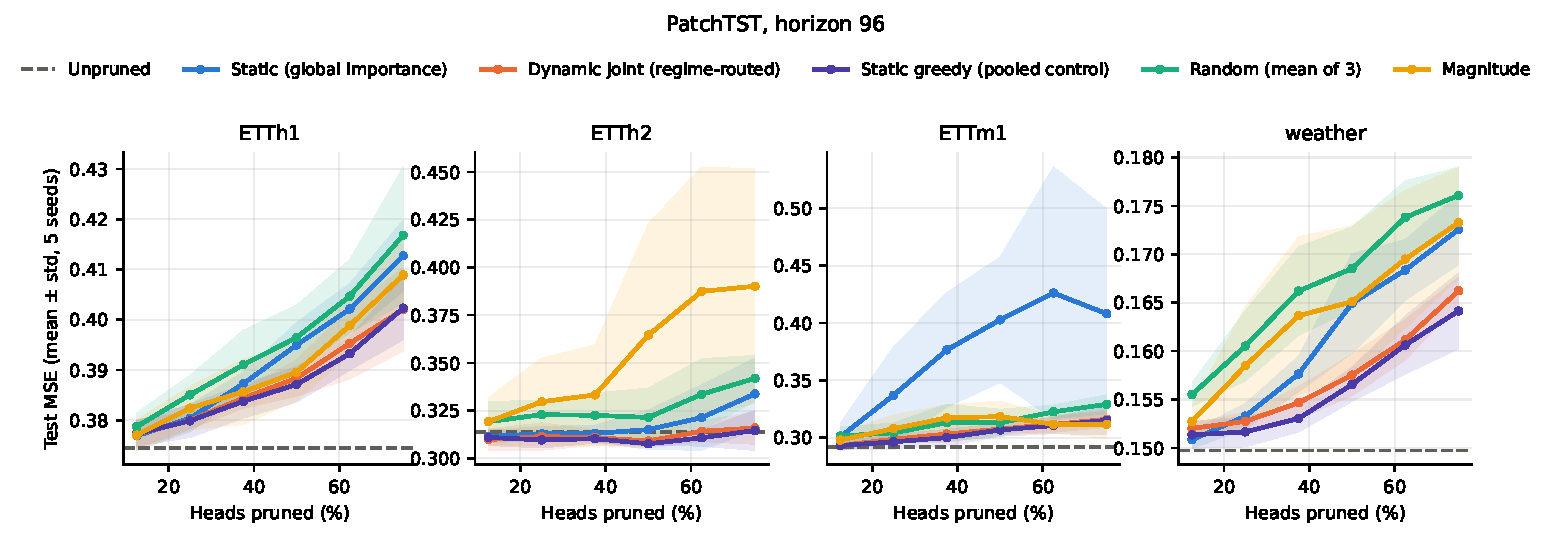
\includegraphics[width=\textwidth]{figures/fig_sweep_patchtst.pdf}
  \caption{Test MSE versus fraction of heads pruned (PatchTST, horizon 96;
  mean $\pm$ std over 5 seeds). The standard independent-importance
  ranking (blue) collapses on ETTm1 --- worse than random --- while both
  greedy variants (orange: per-regime; violet: pooled control) track the
  unpruned baseline (dashed) and degrade gracefully.}
  \label{fig:sweep}
\end{figure*}
% figures/fig_sweep_patchtst.pdf -> \label{fig:sweep}
% figures/fig_all_cells.pdf (appendix) -> \label{fig:allcells}
Figure~\ref{fig:sweep} shows the sparsity sweep at horizon $96$; the full
$16$-cell grid is in Appendix Fig.~\ref{fig:allcells}. The standard
independent-importance ranking is strikingly fragile: on ETTm1 it
degrades test MSE by $+15.4\%$ already at $25\%$ sparsity and by up to
$+46\%$ at deeper cuts --- worse than \emph{random} pruning --- and on
ETTh1@720 it reaches $+164\%$. Both greedy variants (pooled and
per-regime) remain within ${\sim}1\%$ of the unpruned baseline at $25\%$
and degrade gracefully to $75\%$ on every dataset. Magnitude ranking is
consistently weak. Seed-level analysis explains the fragility: the six
lowest-importance heads under independent scoring vary strongly across
seeds, and ignoring head interactions makes the resulting mask
high-variance --- visible as the wide blue uncertainty bands in
Fig.~\ref{fig:sweep}.

\subsection{Attribution: criterion, not conditioning}
\label{sec:results-attribution}

\begin{figure}[!htbp]
  \centering
  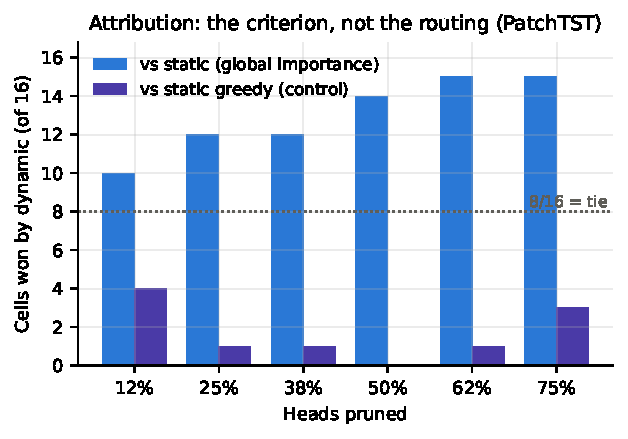
\includegraphics[width=\linewidth]{figures/fig_dose_response.pdf}
  \caption{Attribution across 16 dataset$\times$horizon cells. Dynamic
  regime-routed selection wins up to $15/16$ cells against the standard
  static baseline (blue), but only $0$--$4/16$ against the pooled greedy
  control (violet): the selection criterion, not the regime conditioning,
  explains the gain.}
  \label{fig:dose}
\end{figure}
% figures/fig_dose_response.pdf -> \label{fig:dose}
% figures/fig_bootstrap_forest.pdf (appendix) -> \label{fig:forest}
Against the standard static baseline, regime-routed greedy selection wins
$14/16$ cells at $50\%$ sparsity ($p{=}0.004$) and $15/16$ at
$62.5$--$75\%$ ($p{=}5\times10^{-4}$) --- exactly the kind of result
reported in favour of dynamic pruning. The control reverses it: against
the \emph{pooled} greedy mask, dynamic wins only $0$--$4/16$ cells at any
sparsity (Fig.~\ref{fig:dose}). The apparent advantage of the dynamic
method is explained by its selection criterion; conditioning on the
regime adds selection noise (minority regimes contribute few validation
windows) without adding accuracy. The per-cell bootstrap
(Fig.~\ref{fig:forest}) confirms the picture at $25\%$ sparsity: dynamic
is significantly better than the standard static in $8/16$ cells and
never significantly worse, while static is significantly worse than the
unpruned baseline in $11/16$ cells.

\subsection{The routing headroom is real but aleatoric}
\label{sec:results-routing}

\begin{figure}[!htbp]
  \centering
  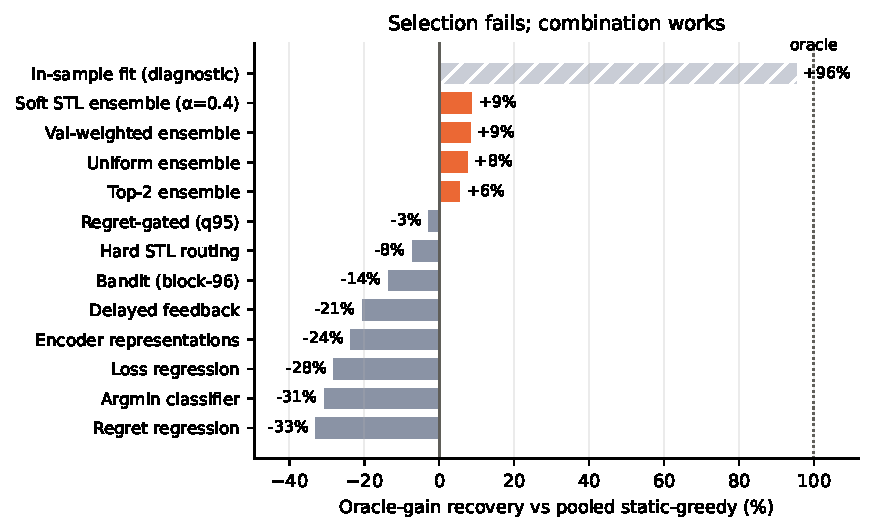
\includegraphics[width=\linewidth]{figures/fig_router_recovery.pdf}
  \caption{Oracle-gain recovery relative to the pooled static-greedy mask.
  Every deployable router (grey) is net negative; prediction ensembles
  (orange) are the only positive deployable methods. The in-sample fit
  (hatched; not deployable) shows the router hypothesis class is
  expressive enough --- the signal, not the model, is what is missing.}
  \label{fig:router}
\end{figure}

\begin{figure}[!htbp]
  \centering
  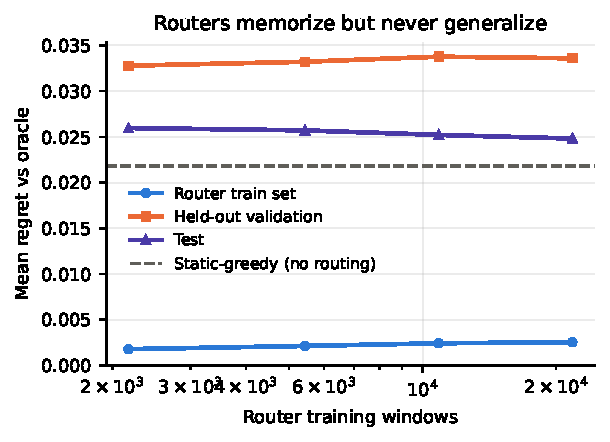
\includegraphics[width=\linewidth]{figures/fig_learning_curve.pdf}
  \caption{Router learning curve (mean over @96 cells). In-sample regret
  stays near zero while held-out validation and test regret remain flat
  --- and above the no-routing reference --- as router training data grows
  $10\times$: routers memorize but never generalize.}
  \label{fig:curve}
\end{figure}
% figures/fig_router_recovery.pdf -> \label{fig:router}
% figures/fig_learning_curve.pdf -> \label{fig:curve}
An oracle routing each test window to its best mask in $\mathcal{M}$
outperforms the \emph{unpruned} model in $15/16$ cells, by up to
$-12.3\%$ (ETTh2@96: $0.2753$ vs $0.3140$) --- a $25\%$-pruned network
contains more usable capacity than the full model, if routed perfectly.
No deployable router captures it (Fig.~\ref{fig:router}): hard STL
routing, the learned detector, four learned oracle-routers,
delayed-feedback and bandit variants, and regret-gating all recover
between $-33\%$ and $-3\%$ of the oracle gain, i.e.\ none beats simply
using the pooled mask ($\leq 6/16$ cells each).

Three diagnostics rule out fixable causes. \emph{Capacity:} fitting the
router in-sample reaches $+96\%$ recovery --- the hypothesis class can
express the routing function. \emph{Data:} with train-split mask losses
added, router training data grows $10\times$ ($2.2$k$\to$$27$k windows)
while held-out regret stays flat (Fig.~\ref{fig:curve}); the router
memorizes its training windows (regret ${\approx}0.002$) at every scale.
\emph{Shift and features:} fitting on the first half of the test set and
predicting the second half fails equally, as does routing from the
model's own mean-pooled encoder representations ($0/4$ datasets). We
conclude the per-window optimal-mask identity is aleatoric at inference
time: it is decided by how a mask's small perturbation interacts with
the unpredictable component of the target.

\subsection{Combination recovers what selection cannot}
\label{sec:results-ensemble}

\begin{figure}[!htbp]
  \centering
  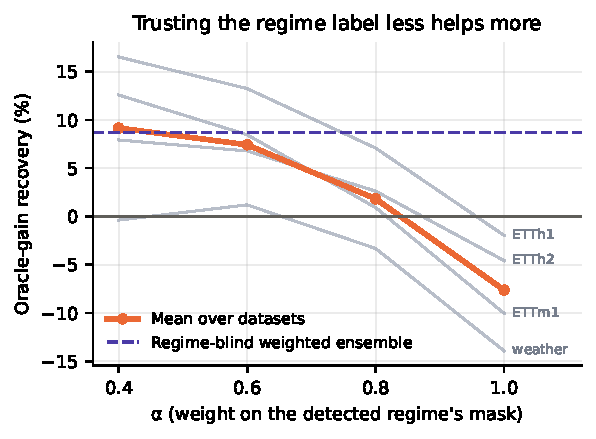
\includegraphics[width=\linewidth]{figures/fig_alpha_sweep.pdf}
  \caption{Soft regime routing: the detected regime's mask receives
  weight $\alpha$, the others share $1{-}\alpha$. Oracle-gain recovery
  falls monotonically as trust in the regime label rises; the best soft
  variants only tie the regime-blind weighted ensemble (dashed).}
  \label{fig:alpha}
\end{figure}
% figures/fig_alpha_sweep.pdf -> \label{fig:alpha}
% figures/fig_diversity_headroom.pdf (appendix) -> \label{fig:diversity}
Averaging the specialist masks' \emph{predictions} sidesteps the
prediction problem. The top-$2$ ensemble (two best masks by validation
MSE; two pruned forward passes) beats the pooled mask on $4/4$ datasets;
inverse-MSE weighting recovers $+8.7\%$ of the oracle gain, ties the
unpruned baseline on ETTm1 ($0.2923$ vs $0.2920$) and beats it on ETTh2
($0.3070$ vs $0.3140$). Soft regime routing interpolates between hard
routing and flat averaging: recovery falls monotonically as trust in the
regime label rises --- $+9.2\%$ at $\alpha{=}0.4$, $+7.4\%$ at $0.6$,
$+1.8\%$ at $0.8$, negative at $\alpha{=}1$ (Fig.~\ref{fig:alpha}) ---
and regime-conditional weights merely tie the regime-blind ensemble.
The diversity ablation (Fig.~\ref{fig:diversity}) completes the
attribution: pools of greedy masks from \emph{random} validation
subsamples ensemble comparably on average ($2/4$ datasets each way; on
ETTm1 the random pool also beats the unpruned baseline, $0.2909$ vs
$0.2920$), but regime pools yield systematically deeper oracles
($4/4$ datasets). Regime information thus contributes \emph{offline}, as
the strongest single source of specialist diversity, while the extra
oracle depth it creates is precisely the aleatoric part that remains
unexploitable.

\subsection{Pruning is free with retraining}
\label{sec:results-scratch}

\begin{figure}[!htbp]
  \centering
  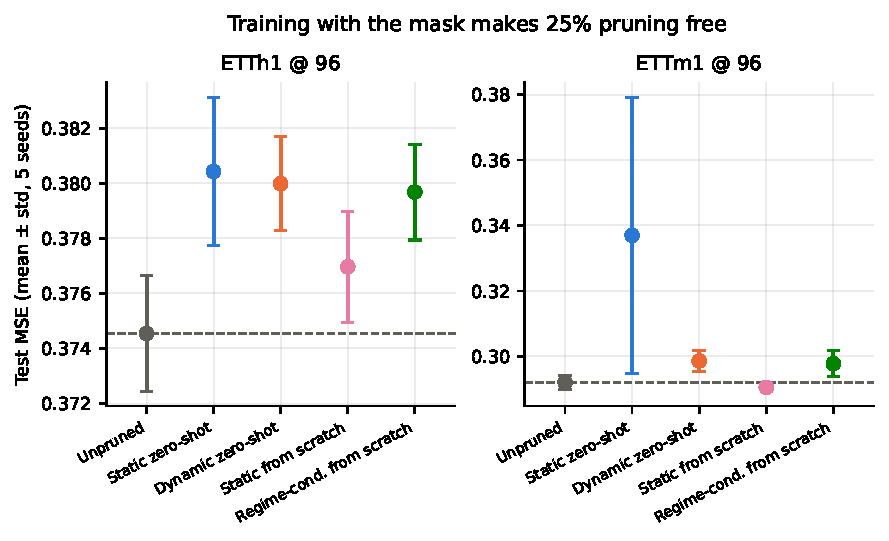
\includegraphics[width=\linewidth]{figures/fig_scratch.pdf}
  \caption{Zero-shot masking versus masked-from-scratch training at
  $25\%$ sparsity (test MSE, mean $\pm$ std over 5 seeds; dashed line =
  unpruned baseline). Training with the mask removes the zero-shot cost
  entirely; the regime-conditional training variant does not improve on
  plain masked training.}
  \label{fig:scratch}
\end{figure}
% figures/fig_scratch.pdf -> \label{fig:scratch}
Imposing the $25\%$ mask from initialization erases the zero-shot cost
entirely (Fig.~\ref{fig:scratch}): scratch-trained static-masked models
reach $0.3770$ vs $0.3745$ unpruned on ETTh1@96 and $0.2905$ vs $0.2920$
(better) on ETTm1@96 --- removing $-5.4\%$ of parameters and $-12\%$ of
FLOPs at no accuracy cost, where zero-shot static pruning had cost up to
$+15\%$. The regime-conditional training variant does not improve on
plain masked training ($0.2977$ vs $0.2905$; a tested negative). This
mirrors lottery-ticket observations \citep{frankle2019lottery}: the
sparsity pattern's value depends on when it is imposed.

\subsection{Generalization to cross-variate attention}
\label{sec:results-itr}

\begin{figure*}[!tp]
  \centering
  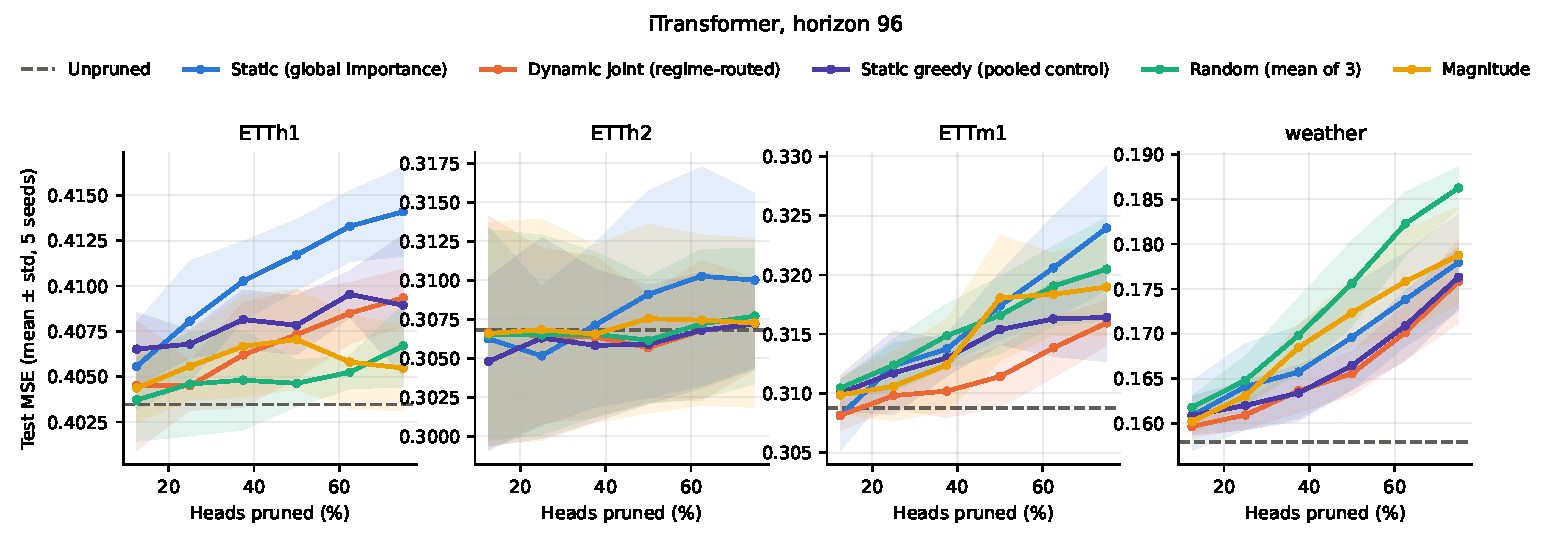
\includegraphics[width=\textwidth]{figures/fig_sweep_itransformer.pdf}
  \caption{The sparsity sweep on iTransformer (horizon 96). Cross-variate
  heads are far more redundant on the 7-variate ETT datasets --- on ETTh2
  pruning improves the model --- while 21-variate Weather shows
  PatchTST-like degradation. The criterion finding replicates; a small
  regime-routing benefit survives the pooled control here, unlike on
  temporal-patch attention.}
  \label{fig:itr}
\end{figure*}
% figures/fig_sweep_itransformer.pdf -> \label{fig:itr}
% figures/fig_arch_comparison.pdf (appendix) -> \label{fig:arch}
On iTransformer at horizon $96$ (Fig.~\ref{fig:itr}), head redundancy is
far larger: on the $7$-variate ETT datasets even $75\%$ pruning costs
only $0.1$--$2.6\%$, and on ETTh2 pruning \emph{improves} the model at
most ratios; only Weather ($21$ variates) shows PatchTST-like
degradation. The criterion finding replicates (independent ranking again
weakest), the oracle again beats the unpruned model on $4/4$ datasets,
and the ensembles again beat the pooled mask. One finding differs:
regime-routed selection beats the pooled control in $4/4$ datasets at
mid sparsities --- small margins on ETT, clearer on Weather
($+1.9\%$ vs $+2.6\%$ at $25\%$ pruning) --- so a modest regime-routing
benefit survives the control on cross-variate attention, plausibly
because regimes alter the between-variable correlation structure these
heads attend to. The aleatoric-routing conclusion therefore applies to
temporal-patch attention, with cross-variate attention marking its
boundary.

\subsection{Deployment notes}
\label{sec:results-deploy}
Per-window STL is the dominant serving cost of any regime-aware policy
($194.5$\,ms/window on CPU); the learned detector reproduces its routing
quality at $4.3$\,ms ($45\times$ faster, $73$--$79\%$ label accuracy,
end-to-end MSE within noise of STL routing). Confidence-aware fallback
to the static mask on ambiguous windows brings no additional gain at any
threshold (Appendix Fig.~\ref{fig:fallback}). The practitioner recipe
implied by our results: prune $25\%$ of heads with pooled greedy
selection and retrain with the mask (free); if accuracy is worth
$2\times$ compute, average the top-$2$ specialist masks; do not build
per-window routers on post-hoc masks.
